\section{Computational Viability}
\label{sec:Results_Computational}

The computational viability of the \ac{eco-glosa} and \ac{flow-glosa} algorithms was assessed by measuring the total simulation runtime for each scenario. Because absolute execution times are hardware-dependent, this analysis focuses primarily on the relative computational overheads between different configurations. The raw durations are listed in Table~\vref{tab:CompViability_TraciComparison} and Table~\vref{tab:CompViability_SumoTraci}.
\mynewline
A primary finding is that the \ac{eco-glosa} algorithm is markedly slower than \ac{flow-glosa}, with the performance gap growing super-linearly with traffic volume, as documented in table~\vref{tab:CompViability_TraciComparison}. At a low demand of $69~\unit{\veh\per\hour}$, the controllers have nearly identical runtimes when no vehicles are equipped. However, at $100\%$ \ac{mpr} under the HBEFA4 model, the \ac{flow-glosa} simulation finishes in $154.27~\unit{\second}$, whereas \ac{eco-glosa} requires $282.56~\unit{\second}$, an increase of $83\%$. This disparity is accentuated by the more demanding PHEMlight5 model, where the slowdown factor reaches $6.2\times$ at full penetration. The performance gap becomes extreme in the saturated scenario of $3462~\unit{\veh\per\hour}$. Here, the \ac{eco-glosa} simulation is over $8.4\times$ slower with HBEFA4 and more than $32\times$ slower with PHEMlight5 compared to its \ac{flow-glosa} counterpart. This significant additional cost is attributable to the fuel-minimisation routine and the high-resolution engine-map lookups that the \ac{eco-glosa} controller must evaluate for every equipped vehicle at each simulation time step.
\mynewline
The choice of simulation interface also introduces a significant bottleneck. A comparison between running \ac{sumo} natively versus controlling it via the \ac{traci} client-server protocol reveals a substantial overhead caused by per-step socket communication, as shown in Table~\vref{tab:CompViability_SumoTraci}. For a low-demand scenario ($69~\unit{\veh\per\hour}$), a \ac{traci}-controlled simulation with the HBEFA4 model takes nearly ten times longer than a native \ac{sumo} run ($154.27~\unit{\second}$ versus $15.77~\unit{\second}$ at $100\%$ \ac{mpr}). In the saturated regime ($3462~\unit{\veh\per\hour}$), the penalty is even more severe. At $100\%$ \ac{mpr} with the HBEFA4 model, the \ac{traci} implementation requires $7670.32~\unit{\second}$, which is over $17\times$ longer than the $450.10~\unit{\second}$ needed for the native run. This demonstrates that the communication overhead of \ac{traci} is a major performance consideration, independent of the controller logic itself.
\mynewline
The graphical results in Figures~\vref{fig:Comp_69} to \vref{fig:Comp_3462} visually confirm these trends. At every demand level, the simulation time for \ac{eco-glosa} increases with a much steeper slope as a function of \ac{mpr} than that of \ac{flow-glosa}, which exhibits a milder, more manageable scaling.

\begin{figure}[htb]
  \centering
  \begin{subfigure}[b]{0.45\textwidth}
    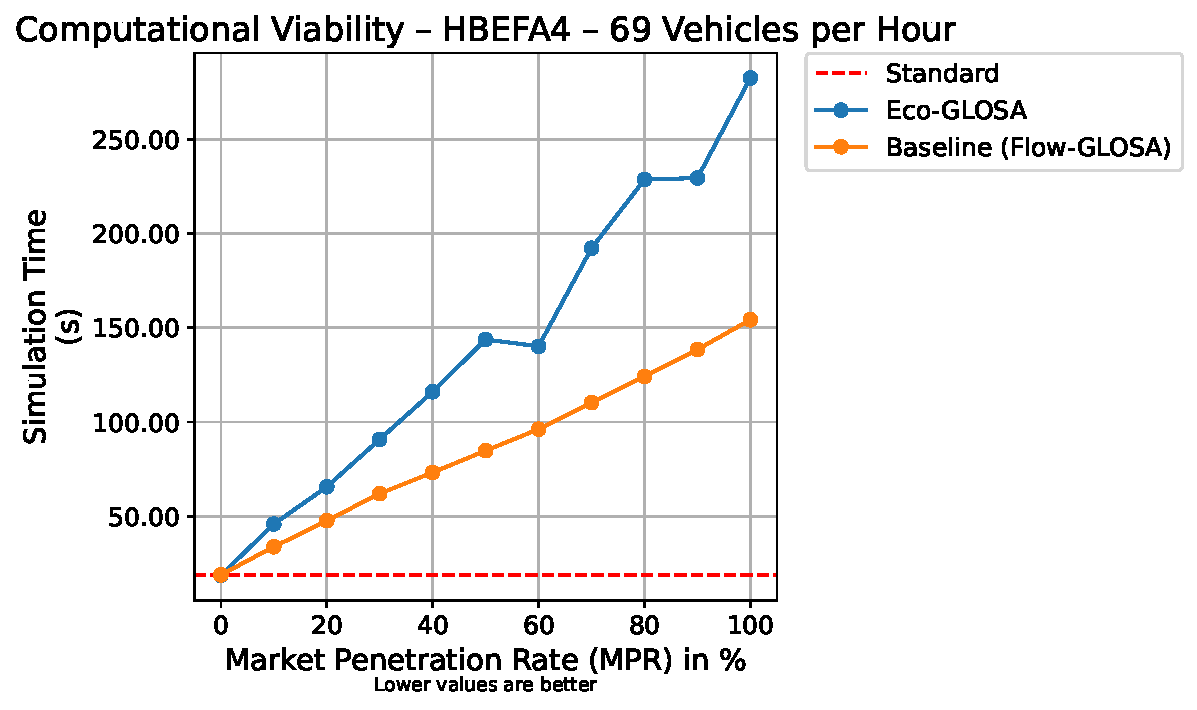
\includegraphics[width=\textwidth]{data/img/ComputationalViability/ComputationalViability_HBEFA4_Cars69.pdf}
    \caption{Runtimes with the HBEFA4 emission model.}
    \label{fig:Comp_69_HBEFA4}
  \end{subfigure}\hfill
  \begin{subfigure}[b]{0.45\textwidth}
    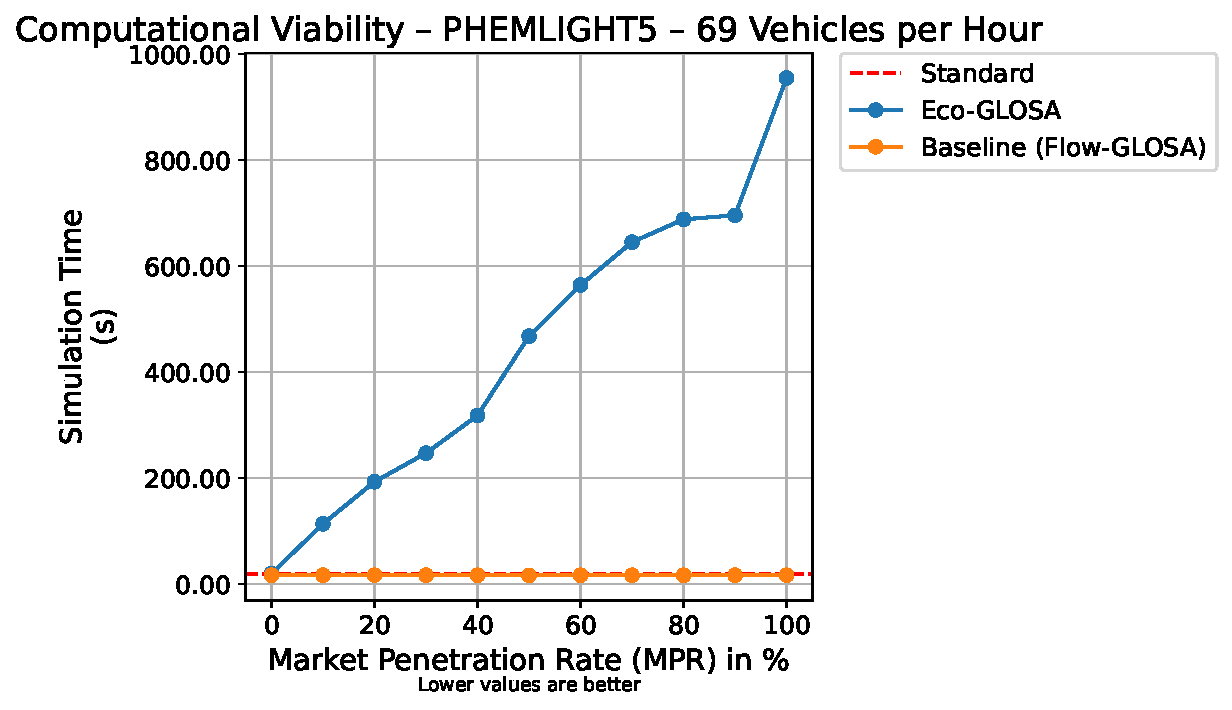
\includegraphics[width=\textwidth]{data/img/ComputationalViability/ComputationalViability_PHEMLIGHT5_Cars69.pdf}
    \caption{Runtimes with the PHEMlight5 emission model}
    \label{fig:Comp_69_PHEM}
  \end{subfigure}
  \caption[Computational Cost at Low Traffic Volume]{A comparison of simulation runtimes as a function of \ac{mpr} at a low traffic volume of $69~\unit{\veh\per\hour}$. The plots illustrate the computational cost for the Standard, \ac{eco-glosa}, and \ac{flow-glosa} controllers.}
  \label{fig:Comp_69}
\end{figure}

\begin{figure}[htb]
  \centering
  \begin{subfigure}[b]{0.45\textwidth}
    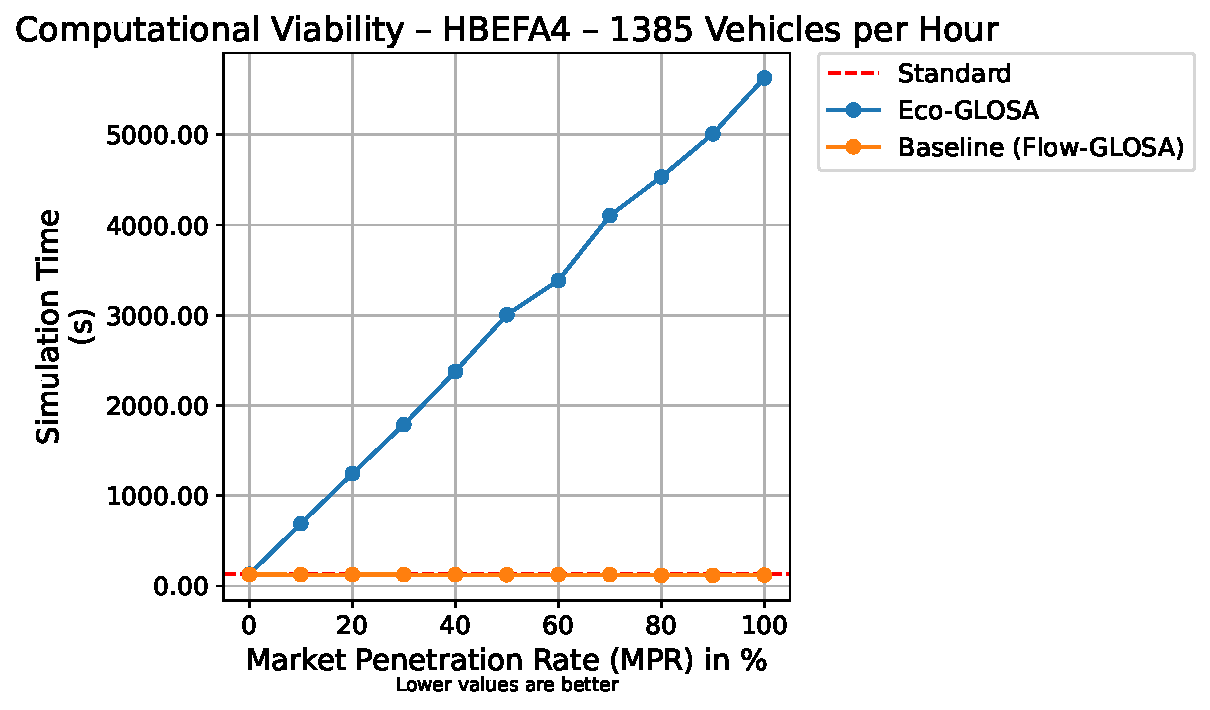
\includegraphics[width=\textwidth]{data/img/ComputationalViability/ComputationalViability_HBEFA4_Cars1385.pdf}
    \caption{Runtimes with the HBEFA4 emission model.}
    \label{fig:Comp_1385_HBEFA4}
  \end{subfigure}\hfill
  \begin{subfigure}[b]{0.45\textwidth}
    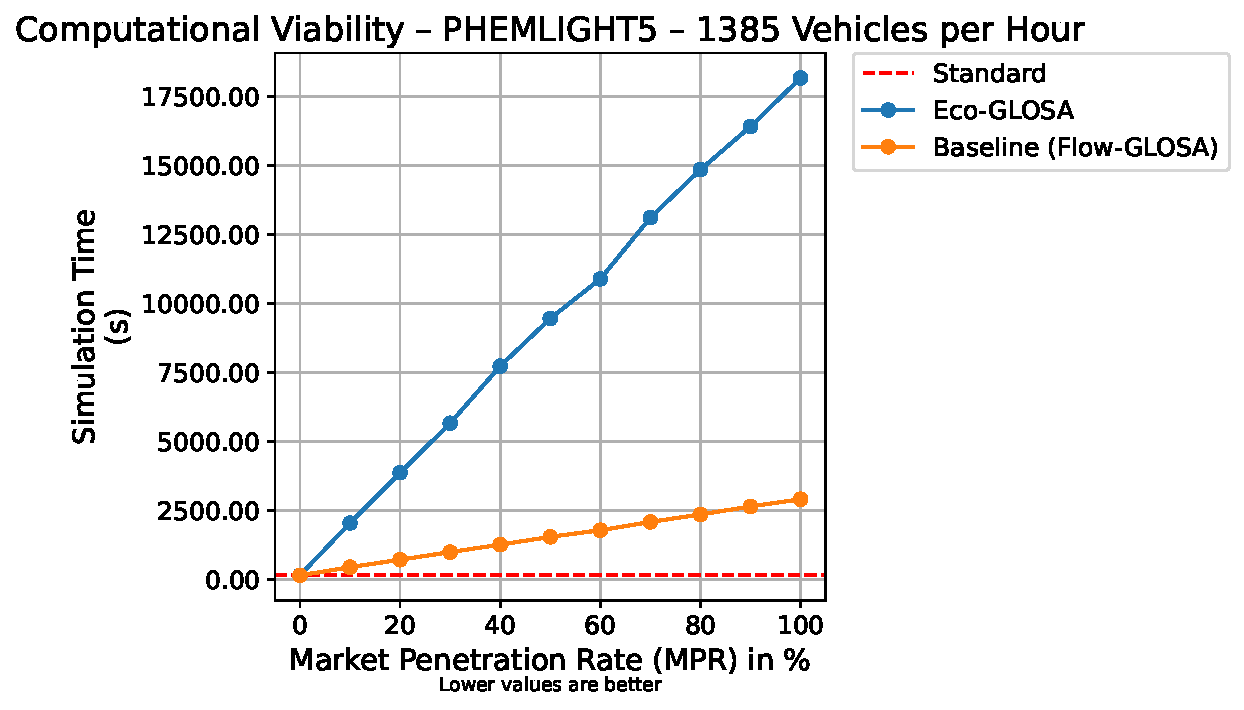
\includegraphics[width=\textwidth]{data/img/ComputationalViability/ComputationalViability_PHEMLIGHT5_Cars1385.pdf}
    \caption{Runtimes with the PHEMlight5 emission model.}
    \label{fig:Comp_1385_PHEM}
  \end{subfigure}
  \caption[Computational Cost at Intermediate Traffic Volume]{Simulation runtimes as a function of \ac{mpr} at an intermediate traffic volume of $1385~\unit{\veh\per\hour}$. The divergence in computational cost between \ac{eco-glosa} and \ac{flow-glosa} becomes more pronounced.}
  \label{fig:Comp_1385}
\end{figure}

\begin{figure}[htb]
  \centering
  \begin{subfigure}[b]{0.45\textwidth}
    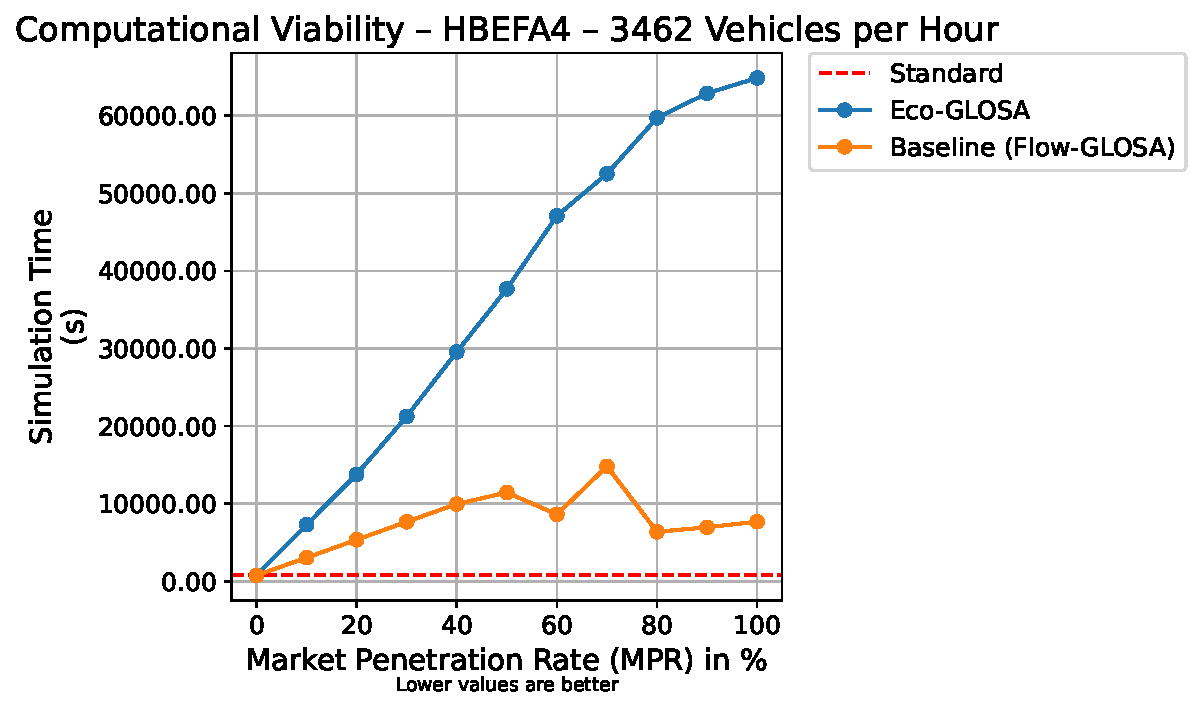
\includegraphics[width=\textwidth]{data/img/ComputationalViability/ComputationalViability_HBEFA4_Cars3462.pdf}
    \caption{Runtimes using the HBEFA4 model.}
    \label{fig:Comp_3462_HBEFA4}
  \end{subfigure}\hfill
  \begin{subfigure}[b]{0.45\textwidth}
    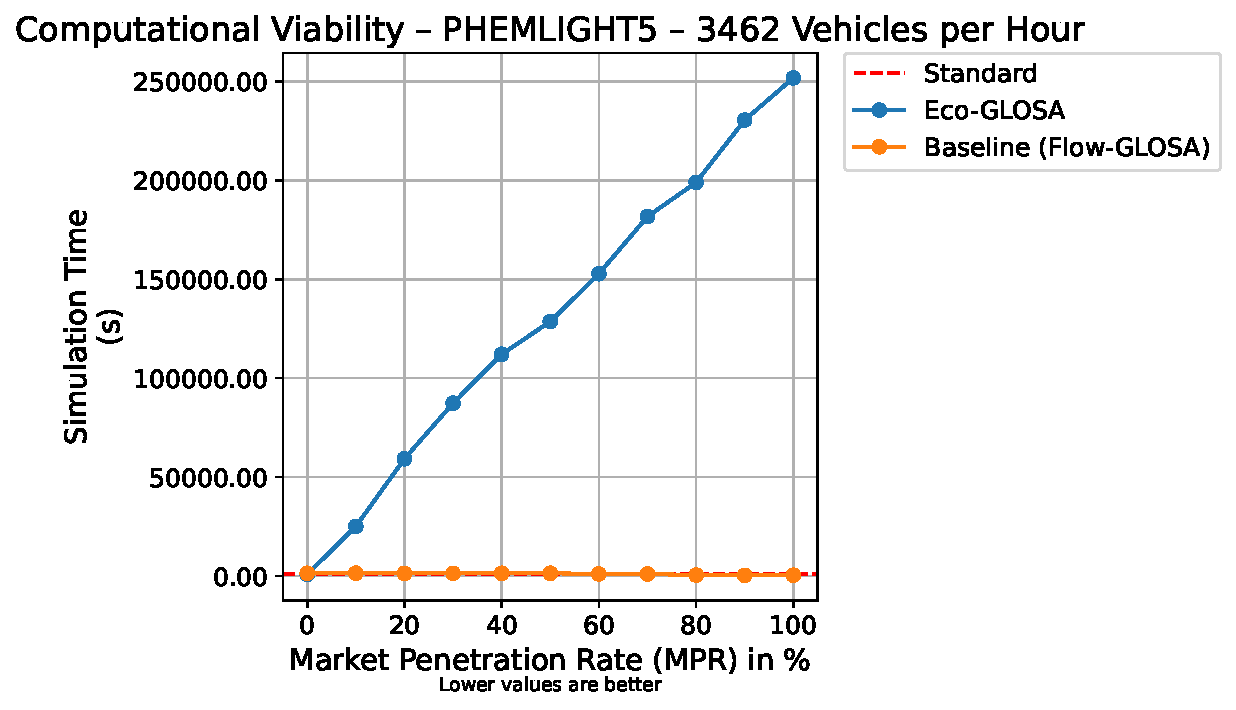
\includegraphics[width=\textwidth]{data/img/ComputationalViability/ComputationalViability_PHEMLIGHT5_Cars3462.pdf}
    \caption{Runtimes using the PHEMlight5 model}
    \label{fig:Comp_3462_PHEM}
  \end{subfigure}
  \caption[Computational Cost in Saturated Conditions]{Simulation runtimes versus \ac{mpr} in the fully saturated regime of $3462~\unit{\veh\per\hour}$. The plots highlight the extreme computational overhead of the \ac{eco-glosa} controller in high-density scenarios.}
  \label{fig:Comp_3462}
\end{figure}

\paragraph{Conclusion on Computational Cost.}
In summary, the \ac{eco-glosa} controller entails a steep computational surcharge, running up to $6\times$ slower than the baseline at low volumes and more than $32\times$ slower in full saturation. Furthermore, the \ac{traci} interface alone imposes an additional slowdown factor of approximately $9\times$ to $17\times$ relative to a native implementation. These findings underline the necessity of using a native \ac{sumo} integration or a dedicated, GPU-accelerated implementation to achieve practical runtimes for complex \ac{eco-glosa} algorithms in large-scale or real-time deployments.

\begin{table}[htb]
  \centering
  \caption[Simulation Runtimes: Controller Comparison]{Absolute simulation runtimes (in seconds) for the \ac{eco-glosa} and \ac{flow-glosa} controllers under the \ac{traci} interface. The data is presented for all traffic volumes and both emission models. Note: absolute times are hardware-dependent.}
  \label{tab:CompViability_TraciComparison}
  \resizebox{\textwidth}{!}{%
    \begin{tabular}{l l l *{11}{c}}
      \toprule
      Vehicles & Algorithm                 & Fuel         & \textbf{0\% (Std.)} & 10\%       & 20\%       & 30\%       & 40\%       & 50\%       & 60\%       & 70\%       & 80\%       & 90\%       & 100\%      \\
      \midrule
      69.0  & Eco-GLOSA                  & HBEFA4       & \textbf{18.64}      & 45.85      & 65.61      & 90.83      & 116.07     & 143.79     & 140.17     & 192.22     & 228.63     & 229.47     & 282.56     \\
      69.0  & Baseline (Flow-GLOSA)      & HBEFA4       & \textbf{18.89}      & 33.81 & 47.66      & 62.03      & 73.24      & 84.78      & 96.20      & 110.26     & 124.18     & 138.50     & 154.27     \\
      69.0  & Eco-GLOSA                  & PHEMlight5   & \textbf{19.79}      & 113.47     & 192.99     & 246.83     & 318.11     & 467.78     & 564.11     & 645.15     & 688.17     & 695.72     & \textbf{954.95} \\
      69.0  & Baseline (Flow-GLOSA)      & PHEMlight5   & \textbf{19.74}      & 35.07      & 48.86      & 62.42      & 74.12      & 86.59      & 97.60      & 111.75     & 126.13     & 139.04     & 153.64     \\
      \midrule
      138.0 & Eco-GLOSA                  & HBEFA4       & \textbf{24.35}      & 71.47      & 109.07     & 147.94     & 199.01     & 276.45     & 271.03     & 374.97     & 429.04     & 476.37     & 538.66     \\
      138.0 & Baseline (Flow-GLOSA)      & HBEFA4       & \textbf{24.51}      & 52.91 & 78.94      & 101.98     & 133.92     & 160.74     & 183.96     & 216.30     & 243.30     & 272.53     & 296.83     \\
      138.0 & Eco-GLOSA                  & PHEMlight5   & \textbf{26.35}      & 167.41     & 324.63     & 393.20     & 508.62     & 859.65     & 808.66     & 1041.76    & 1225.48    & 1519.14    & \textbf{1617.62} \\
      138.0 & Baseline (Flow-GLOSA)      & PHEMlight5   & \textbf{26.35}      & 55.08      & 81.36      & 104.24     & 136.92     & 164.67     & 186.48     & 218.25     & 249.58     & 275.22     & 299.86     \\
      \midrule
      346.0 & Eco-GLOSA                  & HBEFA4       & \textbf{41.48}      & 157.89     & 280.45     & 464.09     & 539.94     & 709.78     & 802.68     & 933.80     & 1062.64    & 1178.17    & 1337.18    \\
      346.0 & Baseline (Flow-GLOSA)      & HBEFA4       & \textbf{41.25}      & 108.99 & 179.65     & 253.48     & 309.06     & 382.80     & 449.63     & 510.24     & 581.60     & 654.66     & 697.96     \\
      346.0 & Eco-GLOSA                  & PHEMlight5   & \textbf{45.96}      & 408.26     & 909.13     & 1422.53    & 1636.71    & 2058.14    & 2573.80    & 2762.42    & 3290.75    & 3709.17    & \textbf{4034.62} \\
      346.0 & Baseline (Flow-GLOSA)      & PHEMlight5   & \textbf{45.96}      & 113.87     & 183.71     & 257.67     & 314.50     & 384.77     & 449.25     & 522.51     & 583.57     & 653.83     & 702.11     \\
      \midrule
      692.0 & Eco-GLOSA                  & HBEFA4       & \textbf{70.06}      & 290.22     & 507.57     & 824.96     & 1077.34    & 1316.33    & 1604.01    & 1844.68    & 2081.46    & 2413.43    & 2689.71    \\
      692.0 & Baseline (Flow-GLOSA)      & HBEFA4       & \textbf{70.01}      & 199.61 & 328.83     & 466.43     & 598.32     & 746.09     & 878.61     & 1009.32    & 1138.79    & 1285.82    & 1423.82    \\
      692.0 & Eco-GLOSA                  & PHEMlight5   & \textbf{79.38}      & 830.27     & 1458.45    & 2363.30    & 3059.37    & 3879.64    & 4721.61    & 5316.79    & 6342.07    & 7676.13    & \textbf{8407.14} \\
      692.0 & Baseline (Flow-GLOSA)      & PHEMlight5   & \textbf{78.96}      & 207.93     & 339.90     & 475.03     & 608.61     & 761.29     & 905.29     & 1024.79    & 1159.32    & 1286.28    & 1435.04    \\
      \midrule
      1385.0& Eco-GLOSA                  & HBEFA4       & \textbf{129.28}     & 690.08     & 1243.97    & 1788.03    & 2377.18    & 3004.73    & 3385.14    & 4103.90    & 4533.56    & 5010.08    & 5629.95    \\
      1385.0& Baseline (Flow-GLOSA)      & HBEFA4       & \textbf{129.45}     & 429.51 & 708.63     & 967.43     & 1238.00    & 1535.47    & 1790.18    & 2092.41    & 2322.02    & 2641.07    & 2872.80    \\
      1385.0& Eco-GLOSA                  & PHEMlight5   & \textbf{149.43}     & 2044.34    & 3869.10    & 5660.32    & 7731.41    & 9458.66    & 10890.27   & 13110.24   & 14853.12   & 16414.57   & \textbf{18175.02} \\
      1385.0& Baseline (Flow-GLOSA)      & PHEMlight5   & \textbf{147.99}     & 443.74     & 714.95     & 990.27     & 1261.04    & 1543.80    & 1784.86    & 2084.13    & 2356.39    & 2643.55    & 2908.28    \\
      \midrule
      2077.0& Eco-GLOSA                  & HBEFA4       & \textbf{194.76}     & 1059.69    & 1975.94    & 2762.06    & 3673.14    & 4655.86    & 5286.35    & 6359.72    & 7099.10    & 8021.73    & 8871.25    \\
      2077.0& Baseline (Flow-GLOSA)      & HBEFA4       & \textbf{192.60}     & 627.27 & 1045.43    & 1477.00    & 1903.69    & 2327.89    & 2743.54    & 3146.68    & 3573.26    & 3965.27    & 4393.02    \\
      2077.0& Eco-GLOSA                  & PHEMlight5   & \textbf{226.03}     & 2940.59    & 5345.12    & 8709.82    & 12229.50   & 14562.74   & 17021.70   & 19812.39   & 22670.23   & 24838.64   & \textbf{27842.28} \\
      2077.0& Baseline (Flow-GLOSA)      & PHEMlight5   & \textbf{222.82}     & 652.90     & 1077.84    & 1530.54    & 1937.15    & 2392.21    & 2784.75    & 3172.89    & 3612.89    & 4026.18    & 4391.33    \\
      \midrule
      2769.0& Eco-GLOSA                  & HBEFA4       & \textbf{265.40}     & 1717.59    & 3066.87    & 9783.80 & 9676.92    & 6817.65    & 29119.22 & 9456.50    & 10410.82   & 11515.24   & 12838.56   \\
      2769.0& Baseline (Flow-GLOSA)      & HBEFA4       & \textbf{263.91}     & 911.38     & 1502.86    & 2086.31    & 2665.99    & 3275.49    & 3829.42    & 4361.18    & 4926.63    & 5492.37    & 5976.06    \\
      2769.0& Eco-GLOSA                  & PHEMlight5   & \textbf{306.78}     & 5033.51    & 18916.38   & 47755.69   & 69552.51   & 94654.61   & 114831.96  & 145268.05  & 142126.60  & 165711.80  & \textbf{139171.65} \\
      2769.0& Baseline (Flow-GLOSA)      & PHEMlight5   & \textbf{305.10}     & 944.66     & 1549.56    & 2131.41    & 2691.56    & 3273.49    & 3865.19    & 4369.02    & 4948.13    & 5467.45    & 6036.59    \\
      \midrule
      3462.0& Eco-GLOSA                  & HBEFA4       & \textbf{762.47}     & 7291.92    & 13774.00   & 21248.52   & 29553.07   & 37682.93   & 47089.12   & 52511.10   & 59711.69   & 62882.26   & 64860.61   \\
      3462.0& Baseline (Flow-GLOSA)      & HBEFA4       & \textbf{753.90}     & 3029.19 & 5342.64    & 7660.62    & 9947.82    & 11430.39   & 8613.54    & 14805.14   & 6367.47    & 6947.72    & 7670.32    \\
      3462.0& Eco-GLOSA                  & PHEMlight5   & \textbf{867.03}     & 25083.58   & 59247.59   & 87348.07   & 112061.03  & 128604.77  & 152756.97  & 181628.56  & 198892.38  & 230399.98  & \textbf{251661.36} \\
      3462.0& Baseline (Flow-GLOSA)      & PHEMlight5   & \textbf{858.37}     & 3133.66    & 5465.48    & 7801.65    & 9987.87    & 11538.38   & 8697.48    & 14902.05   & 6354.86    & 7020.78    & 7713.73    \\
      \bottomrule
    \end{tabular}%
  }
\end{table}

\begin{table}[htb]
  \centering
  \caption[Simulation Runtimes: Native SUMO vs. TraCI]{Comparison of simulation runtimes (in seconds) between a native \ac{sumo} implementation and the \ac{traci} interface for the \ac{flow-glosa} controller. The data illustrates the computational overhead introduced by the external interface.}
  \label{tab:CompViability_SumoTraci}
  \resizebox{\textwidth}{!}{%
    \begin{tabular}{l l l *{11}{c}}
      \toprule
      Cars   & Interface & Fuel         & \textbf{0\% (Std.)} & 10\%       & 20\%       & 30\%       & 40\%       & 50\%       & 60\%       & 70\%       & 80\%       & 90\%       & \textbf{100\%}      \\
      \midrule
      69.0   & \ac{sumo}  & HBEFA4       & \textbf{15.96}      & 15.84      & 15.96      & 15.93      & 15.82      & 15.59      & 15.36      & 15.88      & 15.86      & 15.55      & \textbf{15.77}      \\
      69.0   & \ac{traci} & HBEFA4       & \textbf{18.89}      & 33.81      & 47.66      & 62.03      & 73.24      & 84.78      & 96.20      & 110.26     & 124.18     & 138.50     & \textbf{154.27}     \\
      69.0   & \ac{sumo}  & PHEMlight5   & \textbf{16.64}      & 16.68      & 16.68      & 16.75      & 16.53      & 16.31      & 16.55      & 16.60      & 16.50      & 16.64      & \textbf{16.63}      \\
      69.0   & \ac{traci} & PHEMlight5   & \textbf{19.74}      & 35.07      & 48.86      & 62.42      & 74.12      & 86.59      & 97.60      & 111.75     & 126.13     & 139.04     & \textbf{153.64}     \\
      \midrule
      3462.0 & \ac{sumo}  & HBEFA4       & \textbf{1230.76}    & 1329.20    & 1209.42    & 1251.33    & 1272.75    & 1265.75    & 763.47     & 1027.12    & 574.92     & 322.30     & \textbf{450.10}     \\
      3462.0 & \ac{traci} & HBEFA4       & \textbf{753.90}     & 3029.19    & 5342.64    & 7660.62    & 9947.82    & 11430.39   & 8613.54    & 14805.14   & 6367.47    & 6947.72    & \textbf{7670.32}    \\
      3462.0 & \ac{sumo}  & PHEMlight5   & \textbf{1420.65}    & 1479.41    & 1382.70    & 1406.62    & 1418.44    & 1421.34    & 1071.85    & 1068.90    & 519.48     & 365.01     & \textbf{461.61}     \\
      3462.0 & \ac{traci} & PHEMlight5   & \textbf{858.37}     & 3133.66    & 5465.48    & 7801.65    & 9987.87    & 11538.38   & 8697.48    & 14902.05   & 6354.86    & 7020.78    & \textbf{7713.73}    \\
      \bottomrule
    \end{tabular}%
  }
\end{table}